\documentclass{article}
\usepackage{tikz}
\begin{document}
\begin{center}
\begin{tikzpicture}
<<<<<<< HEAD
\node{Sentence}[sibling distance = 3cm, level distance = 3cm, align=center]
child {node {Unrecognized : garcon}};
=======
\node{S}[sibling distance = 3cm, level distance = 3cm]
child { node {GV} child { node {Sujet} child { node {GN} child { node {Determinant} child {node {ta}}}child {node {}}child { node {Nom} child {node {mère}}}child {node {}}}}child { node {Verbe} child {node {suce}}}};
>>>>>>> refs/remotes/TIPE_Github/main
\end{tikzpicture}
\end{center}
\begin{center}
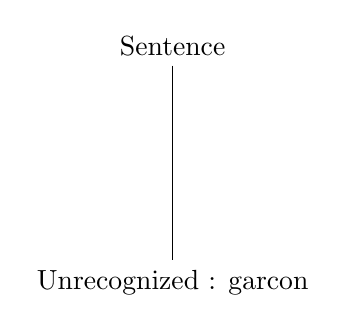
\begin{tikzpicture}
<<<<<<< HEAD
\node{Sentence}[sibling distance = 3cm, level distance = 3cm, align=center]
child {node {Unrecognized : garcon}};
\end{tikzpicture}
\end{center}
\begin{center}
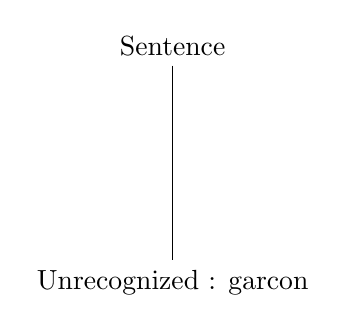
\begin{tikzpicture}
\node{Sentence}[sibling distance = 3cm, level distance = 3cm, align=center]
child {node {Unrecognized : garcon}};
\end{tikzpicture}
\end{center}
\begin{center}
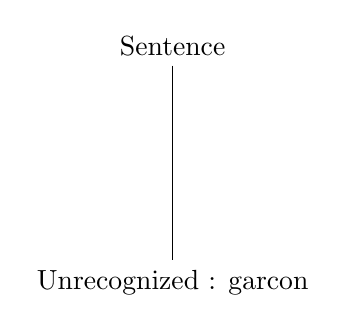
\begin{tikzpicture}
\node{Sentence}[sibling distance = 3cm, level distance = 3cm, align=center]
child {node {Unrecognized : garcon}};
\end{tikzpicture}
\end{center}
\begin{center}
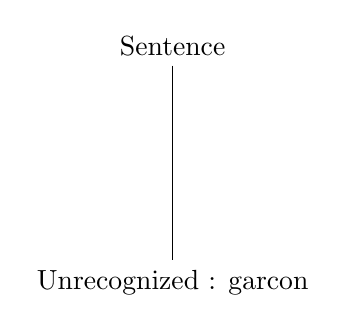
\begin{tikzpicture}
\node{Sentence}[sibling distance = 3cm, level distance = 3cm, align=center]
child {node {Unrecognized : garcon}};
\end{tikzpicture}
\end{center}
\begin{center}
\begin{tikzpicture}
\node{Sentence}[sibling distance = 3cm, level distance = 3cm, align=center]
child {node {Unrecognized : garcon}};
=======
\node{S}[sibling distance = 3cm, level distance = 3cm]
child { node {GV} child { node {Sujet} child { node {GN} child { node {Determinant} child {node {ta}}}child {node {}}child { node {Nom} child {node {mère}}}child {node {}}}}child { node {Verbe} child {node {suce}}}};
>>>>>>> refs/remotes/TIPE_Github/main
\end{tikzpicture}
\end{center}
\end{document}